% CISS 2027 submission draft. Compile with pdflatex (twice).
% If the official IEEEtran.cls is in this folder it is used automatically; otherwise a two-column fallback is used.
% Set \anontrue to hide author names for a double-blind submission.
\newif\ifanon \anonfalse
\newif\ifieee
\IfFileExists{IEEEtran.cls}{\ieeetrue\documentclass[conference]{IEEEtran}}{\ieeefalse\documentclass[10pt,twocolumn,letterpaper]{article}}
\ifieee\else
  \usepackage[letterpaper,left=0.75in,right=0.75in,top=0.75in,bottom=1.0in,columnsep=0.25in]{geometry}
  \usepackage{mathptmx}
  \providecommand{\IEEEauthorblockN}[1]{\large #1\\[3pt]}
  \providecommand{\IEEEauthorblockA}[1]{\normalsize\itshape #1}
  \date{}
  \newenvironment{IEEEkeywords}{\noindent\textit{Keywords---}}{\par}
  \renewcommand{\abstractname}{}
\fi
\usepackage[T1]{fontenc}
\usepackage[utf8]{inputenc}
\usepackage{booktabs,graphicx,amsmath,amssymb,url,microtype,multirow,array}
\usepackage[hidelinks]{hyperref}
\urlstyle{same}
\setlength{\tabcolsep}{3.2pt}
\begin{document}
\title{Beyond Accuracy: Answer Leakage and Prompt Structure in LLM Diagnostic Reasoning on MedR-Bench}
\ifanon
  \author{\IEEEauthorblockN{Anonymous Authors}}
\else
  \author{\IEEEauthorblockN{Akshay Bhuvaneswari Ramakrishnan and Meenalosini Vimal Cruz}
  \IEEEauthorblockA{School of Computing, Allen E.\ Paulson College of Engineering and Computing\\
  Georgia Southern University, Statesboro, GA 30460, USA}}
\fi
\maketitle
\ifieee\else\thispagestyle{empty}\fi

\begin{abstract}
Clinical language models and the prompts used with them are usually compared on final-diagnosis accuracy. We argue that this endpoint can mislead in two ways: published case reports can state the answer, and a correct label says nothing about the reasoning behind it. We tested both on 120 MedR-Bench diagnosis cases (70 rare, 50 common), crossing three prompt styles (bare, stepwise, structured) with Claude Opus 5.5 and Gemini 4 Neon on text from which statements of the diagnosis had been redacted, and re-running the bare prompt on the original text. Restoring the redacted statements raised strict accuracy by 19.2 points for Claude and 16.7 for Gemini (Holm-adjusted $p<0.001$), almost entirely in the redacted cases. Prompt style moved accuracy by at most 5.8 points, and no style contrast survived correction. The explanation changed far more: structured responses covered 41\% and 61\% of the clinician's reference reasoning steps after length correction, against 18\% and 29\% for stepwise responses (paired $p<10^{-18}$). On a 40-case subset, two LLM judges from untested families rated reasoning soundness. One found structured reasoning sounder for both models (Gemini 67.5\% to 85.0\%, $p=0.016$); the other found almost no change. Accuracy alone overstated the models and hid most of the prompt effect.
\end{abstract}
\begin{IEEEkeywords}
large language models, clinical diagnosis, diagnostic reasoning, prompt engineering, data leakage, LLM evaluation
\end{IEEEkeywords}

\section{Introduction}
Language models are increasingly compared, and their prompts chosen, by how often the final diagnosis matches an answer key. That endpoint has two blind spots. First, many benchmarks are built from published case reports written after the diagnosis was known, and the text can state the answer or imply it through later results or treatment. Yang et al.\ found that appending treatment records to rare-disease narratives raised Recall@1 by 15.3 points \cite{yang2026}. Second, a correct label says nothing about how it was reached. Written explanations need not reflect the cause of an answer \cite{turpin2023}, and on MedR-Bench model reasoning is generally factual but often misses critical steps \cite{qiu2025}.

Both blind spots matter for prompt comparisons. If part of the text leaks the answer, accuracy sits near a ceiling that no prompt controls. If a prompt changes the reasoning but not the label, an accuracy-only comparison reports no effect. In an earlier pilot on MedR-Bench we saw this pattern: accuracy was flat across prompt styles while Gemini's reasoning was rated sound in 72\% of cases under a stepwise prompt and 88\% under a structured work-up. That pilot had one rater, 40 rated cases and no control for leakage.

Here we test the idea on a clean rerun. We ask: (i) how much of measured accuracy depends on statements of the diagnosis in the text, (ii) how much prompt style changes accuracy once those statements are removed, and (iii) how much it changes the explanation, measured as coverage of the clinician's reference reasoning and as rated soundness. Our contributions are:
\begin{itemize}
\item A redaction protocol and case-level audit for MedR-Bench, with a paired estimate of the leakage effect and an unmodified-case negative control.
\item Paired, multiplicity-corrected estimates of prompt-style effects on accuracy, explanation coverage and reasoning soundness on the same cases.
\item A grader-robustness analysis for accuracy and a two-judge design for soundness, reported with their disagreement.
\end{itemize}

\section{Related Work}
\textbf{Prompts and diagnostic accuracy.} A structured two-step prompt raised Claude 3.5 Sonnet's accuracy on 322 Diagnosis Please cases from 56.5\% to 60.6\% ($p=0.042$) \cite{sonoda2025}. Other studies find no consistent gain: MedPrompt variants had mixed or adverse effects across 36 cases \cite{chai2025}, chain-of-thought lowered MedGemma's accuracy by 5.7\% \cite{sadanandan2026}, and five prompting techniques did not differ for headache classification \cite{zwanzig2026}. Our accuracy results sit with this mixed evidence; we offer one reason it is mixed.

\textbf{Explanation and reasoning quality.} Savage et al.\ showed that GPT-4 can be prompted to imitate clinical reasoning without losing accuracy \cite{savage2024}, and Hassanein et al.\ found that prompt design shaped both accuracy and expert-rated explanation quality for oral lesions \cite{hassanein2026}. MedR-Bench scores reasoning against clinician-written references \cite{qiu2025}. LLM evaluators of reasoning are themselves fallible: in one study a GPT-4o evaluator failed to discern differences that clinicians saw \cite{liu2026}. We measure explanation quality on the same cases as accuracy and leakage, and use two judges so that their disagreement is visible.

\textbf{Leakage and hindsight.} RareArena separates rare-disease screening, before confirmatory tests, from confirmation with complete information \cite{chen2026}; MMRareBench applies track-specific leakage control \cite{ning2026}; and Matsuura et al.\ show that retrospective records can reward use of future information \cite{matsuura2026}. Yang et al.\ propose programmatic sanitisation of narratives \cite{yang2026}. We apply a redaction audit to MedR-Bench and place its effect next to prompt effects.

\section{Methods}
\subsection{Cases and redaction}
We drew a stratified random sample of 70 rare and 50 common cases (seed 42) from the MedR-Bench diagnosis subset (957 cases, 491 rare) in its oracle setting, which includes ancillary test results \cite{qiu2025}, and split them into 15 fixed batches of eight. Each case was screened with curated patterns for the reference diagnosis in a conclusion (``confirmed X'', ``consistent with X''), an identified organism, gene or tumour type, or a diagnosis component stated as a result; matches were replaced by \texttt{[REDACTED]}. A second pass against the reference labels removed residual statements in nine more cases. In total 56 cases were redacted, 42 had no match, and 22 were kept unchanged (11 where an imaging finding is itself the label, 5 where the diagnosis appears only as prior history, 6 false positives). Before redaction 15 cases contained the full reference label verbatim, and after it none did; partial or paraphrased cues may remain.

\subsection{Prompts, models and procedure}
All prompts shared one instruction (use only the case, no tools, answer all eight cases in order). S1 (bare) asked for the final diagnosis only. S2 (stepwise) asked for step-by-step reasoning, then the diagnosis. S3 (structured) required key findings, a ranked differential of three to five candidates, evidence for and against each, exclusions and commitment, then the diagnosis. Arm A used redacted text with S1--S3; Arm B used original text with S1 only. We used the chat interfaces of Claude Opus 5.5 (medium effort) and Gemini 4 Neon (medium thinking) in November 2026, each batch in a new temporary chat with no tools: 90 Arm A and 30 Arm B runs. Style blocks ran S1--S3 for Claude and S3--S1 for Gemini, with batch order randomised within blocks. Temperature and seed cannot be set in these interfaces, and each condition was run once.

\subsection{Endpoints}
\textbf{Accuracy.} For each case the eight outputs (2 models $\times$ 4 conditions) were shuffled, labelled a--h and graded against the reference by a Claude-family LLM, blind to condition: 2 (strict) for the same primary entity, allowing synonyms and minor detail; 1 (lenient only) for the right family or one component of a multi-part diagnosis; 0 otherwise. Because the grader shares a family with one tested model, a different-family LLM (DeepSeek) re-graded 180 blinded items, comprising every answer graded 1 plus 60 random others, and we repeated the main contrasts under judge-adjusted, conservative and two scripted scorings.

\textbf{Explanation coverage.} MedR-Bench gives a clinician-written reasoning for each case as a list of steps. For each S2 and S3 response, with the final-diagnosis line removed, a step counted as covered when at least half of its content-word stems appeared in the response. To correct for length (S3 is three to four times longer), we subtracted a permutation null: the mean coverage of the same response against 20 other cases' reference steps. We also report the share of strictly correct answers with corrected coverage below 0.10 (thin explanations). Coverage is a lexical proxy for evidence and completeness, close to the completeness dimension of the MedR-Bench evaluator \cite{qiu2025}; it does not measure validity.

\textbf{Reasoning soundness.} For 40 cases sampled at random (23 rare, 17 common), the 160 S2 and S3 responses were stripped of field labels, given random IDs and rated 0/1/2 by two LLMs from families not under test, ChatGPT (OpenAI) and DeepSeek, through their free web interfaces in November 2026. Each item showed the redacted case, the reference diagnosis, the clinician's reference reasoning and the response. The rubric was the pilot's: 2 for sound (decisive findings, valid logic consistent with the reference, main alternatives excluded with appropriate evidence, no material error); 1 for partial; 0 for unsound. Judges were told not to reward length or format and that a wrong diagnosis cannot score 2. %% [ANCHOR PLACEHOLDER: one author rated 30 of the 160 items blind; agreement with each judge is reported in Section IV-D.]

\subsection{Statistics}
Conditions are compared on the same cases. For accuracy we use exact McNemar tests \cite{mcnemar1947} with Holm correction \cite{holm1979} within the four style contrasts and within the two leakage contrasts, separately for strict and lenient scoring, and 95\% Wilson intervals \cite{wilson1927}. Coverage and soundness (S3 versus S2) use Wilcoxon signed-rank tests per model; agreement uses Cohen's $\kappa$ \cite{cohen1960}, weighted $\kappa$ and adjacent agreement, noting that $\kappa$ understates agreement when ratings cluster at the top \cite{liu2026}. Models and styles are never pooled in inferential tests.

\section{Results}
\subsection{Accuracy and the effect of leakage}
On redacted text with the bare prompt, strict accuracy was 70.0\% for Claude and 65.8\% for Gemini (Table~\ref{tab:acc}, Fig.~\ref{fig:acc}). On the original text it was 89.2\% and 82.5\%: +19.2 points (25 cases gained, 2 lost) and +16.7 points (23 gained, 3 lost), both Holm-adjusted $p<0.001$ (Table~\ref{tab:con}). The gain lay in the 56 redacted cases (Claude 53.6\% to 92.9\%; Gemini 55.4\% to 83.9\%). In the 42 cases with no match, whose text was identical in both arms, accuracy changed by $-4.8$ and 0 points; correctness flipped between sessions in 2 and 4 of these 42 cases, our estimate of run-to-run variation. The gain was similar in rare and common cases and in the 34 cases containing therapy or outcome phrases.

\begin{table}[t]
\centering\caption{Accuracy (\%) with 95\% Wilson CI, 120 cases per cell.}\label{tab:acc}
\footnotesize
\begin{tabular}{@{}llcc@{}}
\toprule
Model & Condition & Strict [CI] & Lenient [CI]\\
\midrule
Claude & S1 bare & 70.0 [61,77] & 85.0 [78,90]\\
Claude & S2 stepwise & 72.5 [64,80] & 87.5 [80,92]\\
Claude & S3 structured & 75.8 [67,83] & 90.0 [83,94]\\
Claude & S1, original text & 89.2 [82,94] & 95.0 [90,98]\\
Gemini & S1 bare & 65.8 [57,74] & 89.2 [82,94]\\
Gemini & S2 stepwise & 67.5 [59,75] & 88.3 [81,93]\\
Gemini & S3 structured & 70.8 [62,78] & 88.3 [81,93]\\
Gemini & S1, original text & 82.5 [75,88] & 94.2 [88,97]\\
\bottomrule
\end{tabular}
\end{table}

\begin{figure}[t]
\centering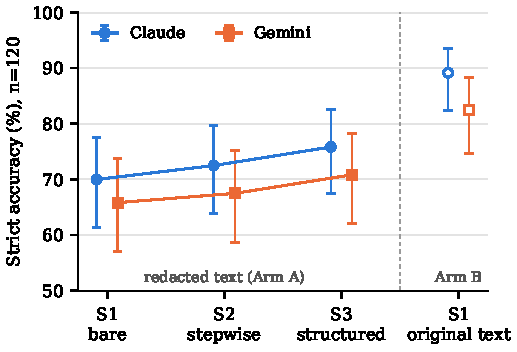
\includegraphics[width=\columnwidth]{fig1.pdf}
\caption{Strict accuracy with 95\% Wilson intervals. Filled markers: redacted text (Arm A); open markers: original text (Arm B, S1 only).}\label{fig:acc}
\end{figure}

\begin{table*}[t]
\centering\caption{Paired accuracy contrasts (points). Gain/loss = cases correct only in the second/first condition; $p$ = exact McNemar; $p_{\mathrm{H}}$ = Holm-adjusted within each block.}\label{tab:con}
\footnotesize
\begin{tabular}{@{}llrcrrrr@{}}
\toprule
 & & \multicolumn{4}{c}{Strict} & \multicolumn{2}{c}{Lenient}\\
\cmidrule(lr){3-6}\cmidrule(lr){7-8}
Model & Contrast & $\Delta$ & gain/loss & $p$ & $p_{\mathrm{H}}$ & $\Delta$ & $p_{\mathrm{H}}$\\
\midrule
Claude & S2 $-$ S1 & +2.5 & 3/0 & 0.250 & 0.500 & +2.5 & 0.750\\
Claude & S3 $-$ S1 & +5.8 & 9/2 & 0.065 & 0.262 & +5.0 & 0.125\\
Gemini & S2 $-$ S1 & +1.7 & 4/2 & 0.688 & 0.688 & -0.8 & 1.000\\
Gemini & S3 $-$ S1 & +5.0 & 7/1 & 0.070 & 0.262 & -0.8 & 1.000\\
\midrule
Claude & Original $-$ redacted (S1) & +19.2 & 25/2 & <0.001 & <0.001 & +10.0 & 0.004\\
Gemini & Original $-$ redacted (S1) & +16.7 & 23/3 & <0.001 & <0.001 & +5.0 & 0.146\\
\bottomrule
\end{tabular}
\end{table*}

\subsection{Prompt style and accuracy}
S3 scored 5.8 points above S1 for Claude (9 gained, 2 lost; $p=0.065$) and 5.0 for Gemini (7 gained, 1 lost; $p=0.070$), both $p_{\mathrm{H}}=0.262$; S2 differed from S1 by 2.5 and 1.7 points. Only 11 (Claude) and 9 (Gemini) of 120 cases changed correctness across styles. The S3 advantage is in the same direction as Sonoda et al.\ \cite{sonoda2025} and of similar size, but our sample cannot resolve it. It is also grader-dependent: the leakage gain stayed between +6.7 and +19.2 points under all five accuracy scorings, whereas S3 minus S1 ranged from $-11.7$ to $+7.5$. The cross-family re-grade agreed with the primary grades on 74\% of the 180 audited items ($\kappa=0.52$; 99\% within one level), being more lenient at the strict boundary.

\subsection{Explanation coverage}
Structure changed the explanation far more than the score (Table~\ref{tab:cov}). After length correction, S3 covered 41.2\% of reference steps for Claude against 18.1\% for S2 (higher in 102 of 120 cases, lower in 15; $p=3\times10^{-19}$) and 61.4\% against 28.5\% for Gemini (112 higher, 7 lower; $p=6\times10^{-21}$), while accuracy rose 3.3 points for each. The gap held among cases correct under both styles (+25.1 and +32.0 points). Among correct answers, thin explanations fell from 37\% to 5\% (Claude) and from 10\% to 0\% (Gemini). Within S3, longer responses were slightly less often correct (Spearman $\rho=-0.19$ and $-0.18$), so length does not explain the S3 accuracy gap.

\begin{table}[t]
\centering\caption{Explanation coverage (redacted text, 120 cases). Words: explanation length. Coverage: \% of reference steps covered, raw and null-corrected. Thin: \% of correct answers with corrected coverage $<$10\%.}\label{tab:cov}
\footnotesize
\begin{tabular}{@{}llccccc@{}}
\toprule
Model & Style & Acc. & Words & Raw & Corr. & Thin\\
\midrule
Claude & S2 stepwise & 72.5 & 87 & 18.2 & 18.1 & 37\\
Claude & S3 structured & 75.8 & 260 & 42.7 & 41.2 & 5\\
\midrule
Gemini & S2 stepwise & 67.5 & 104 & 28.7 & 28.5 & 10\\
Gemini & S3 structured & 70.8 & 451 & 63.8 & 61.4 & 0\\
\bottomrule
\end{tabular}
\end{table}

\subsection{Reasoning soundness}
The two judges agreed exactly on 77\% of the 160 items and never differed by two levels ($\kappa=0.48$; linear-weighted 0.58; sound versus not 0.68). ChatGPT was the stricter judge (lower on 27 items, higher on 10). Table~\ref{tab:snd} gives the share rated sound. Under DeepSeek, S3 was sounder than S2 for both models: 6 Claude cases improved and none worsened ($p=0.031$), and 7 Gemini cases improved and none worsened ($p=0.016$), with Gemini rising from 67.5\% to 85.0\%. Under ChatGPT, 1--2 cases improved and 0--1 worsened per model, not significant. Averaging the judges, S3 minus S2 was +0.11 points on the 0--2 scale for Gemini ($p=0.020$) and +0.08 for Claude ($p=0.070$); after Holm correction over the two models these are 0.039 and 0.070. Soundness was unrelated to explanation length within each style (Spearman $\rho=-0.08$ and $0.04$), so the judges did not visibly reward length. Few correct answers were rated unsound: 7--15\% under S2 and 0--8\% under S3, depending on model and judge. %% [ANCHOR RESULT PLACEHOLDER]

\begin{table}[t]
\centering\caption{Reasoning soundness on 40 cases: \% rated sound (2) with 95\% Wilson CI, by judge. Acc.: strict accuracy on the same 40 cases. Both: rated sound by both judges.}\label{tab:snd}
\footnotesize\setlength{\tabcolsep}{2.4pt}
\begin{tabular}{@{}llcccc@{}}
\toprule
Model & Style & Acc. & ChatGPT & DeepSeek & Both\\
\midrule
Claude & S2 stepwise & 67.5 & 67.5 [52,80] & 60.0 [45,74] & 55.0\\
Claude & S3 structured & 70.0 & 70.0 [55,82] & 75.0 [60,86] & 70.0\\
\midrule
Gemini & S2 stepwise & 57.5 & 72.5 [57,84] & 67.5 [52,80] & 60.0\\
Gemini & S3 structured & 62.5 & 75.0 [60,86] & 85.0 [71,93] & 75.0\\
\bottomrule
\end{tabular}
\end{table}

\section{Discussion}
Accuracy, the endpoint most prompt comparisons use, was the least informative one here. It moved by about 17 to 19 points when statements of the diagnosis were restored, about three times the largest style gap, and by at most 5.8 points across prompt styles. The explanation moved much more: structured prompts more than doubled coverage of the clinician's reference reasoning and nearly removed correct answers with thin explanations. On soundness the evidence is weaker but in the same direction: no model and judge showed S3 less sound than S2, one judge found a clear gain for both models, and the other found almost none.

Against our pilot, the result is a partial replication. The flat accuracy and the size of Gemini's soundness gain under one judge (67.5\% to 85.0\%, against 72\% to 88\% in the pilot) recur. Two things do not. Claude's reasoning was not at ceiling once leaked statements were removed (60--75\% sound), and Claude also improved under that judge, so we do not find the model-dependent effect the pilot suggested. The pilot's near-ceiling accuracy is consistent with our original-text arm (82--89\%) and probably reflected leakage in part.

These results suggest one reason the prompt literature is mixed \cite{sonoda2025,chai2025,sadanandan2026,zwanzig2026}: on case-report text, accuracy sits near a ceiling set partly by the text itself, so style effects are small and noisy, while the larger effects are in the explanation \cite{savage2024,hassanein2026}. For evaluating prompts for clinical LLMs we suggest three practices: report a leakage-sensitivity arm, with an unmodified stratum as a negative control; report at least one explanation endpoint next to accuracy; and when LLMs grade, use more than one and report their disagreement, since our two judges led to different conclusions on soundness.

\subsection{Limitations}
\textbf{Leakage.} Redaction also removed some legitimate findings (for example organism names given as test results), so the Arm B$-$A gain is an upper bound on pure leakage. Partial cues remain, and models saw the \texttt{[REDACTED]} token (in 10 Claude and 4 Gemini output files). Arm B used S1 only, so we cannot test whether leakage interacts with style.
\textbf{Design.} Each condition was run once through consumer chat interfaces without temperature or seed control; style order was fixed per model; batches of eight may allow cross-case effects, and batch size was not varied. The two models are not capability-matched. The sample is 120 English cases from one case-report benchmark.
\textbf{Endpoints.} Accuracy was graded by a Claude-family LLM, checked on 180 items by one other family. Coverage is lexical and rewards restating case findings; structure and length cannot be separated. Soundness was rated on 40 cases by two LLM judges whose versions were not displayed by their interfaces; structured responses remain recognisable after label stripping; and the judges disagreed on the main contrast. %% [Replace with anchor result, or state: no human rated soundness in this study.]
Reference reasoning reflects one clinician's account. We did not assess faithfulness of explanations \cite{turpin2023}.

\section{Conclusion}
On 120 MedR-Bench cases, restoring redacted statements of the diagnosis raised accuracy by 17 to 19 points, while prompt structure moved accuracy by at most 6 points but more than doubled the share of reference reasoning that explanations covered, and improved rated soundness under one of two judges. Evaluations of clinical prompts that report accuracy alone can overstate the model and miss most of the prompt's effect. Future work should add original-text arms for all styles, repeated runs, more models, and blinded clinician ratings of soundness.

\ifanon\else
\section*{Data availability}
Redacted case texts, prompts, raw outputs, grades and analysis scripts will be released at the project repository (github.com/AkshayBRamki/Prompt-Structure).
\fi

\begin{thebibliography}{99}
\bibitem{qiu2025} P.~Qiu \emph{et al.}, ``Quantifying the reasoning abilities of LLMs on clinical cases,'' \emph{Nat.\ Commun.}, vol.~16, art.~9799, 2025.
\bibitem{yang2026} J.~Yang \emph{et al.}, ``Auditing evaluation artifacts and data leakage in large language model systems for rare disease diagnosis,'' arXiv:2610.33592, Oct.\ 2026.
\bibitem{turpin2023} M.~Turpin, J.~Michael, E.~Perez and S.~R.~Bowman, ``Language models don't always say what they think: unfaithful explanations in chain-of-thought prompting,'' in \emph{Adv.\ Neural Inf.\ Process.\ Syst.}, vol.~36, 2023.
\bibitem{sonoda2025} Y.~Sonoda \emph{et al.}, ``Structured clinical reasoning prompt enhances LLM's diagnostic capabilities in diagnosis please quiz cases,'' \emph{Jpn.\ J.\ Radiol.}, vol.~43, pp.~586--592, 2025.
\bibitem{chai2025} M.~Chai and A.~R.~Zomorrodi, ``Prompt engineering does not universally improve large language model performance across clinical decision-making tasks,'' arXiv:2512.22966, 2025.
\bibitem{sadanandan2026} B.~Sadanandan and V.~Behzadan, ``When chain-of-thought backfires: evaluating prompt sensitivity in medical language models,'' arXiv:2603.25960, Mar.\ 2026.
\bibitem{zwanzig2026} D.~Zwanzig, ``Benchmarking prompting strategies for open-source language models in ICHD-3 headache classification,'' in \emph{Health Sciences Informatics Leads and Empowers the Digital Health Transformation}, IOS Press, 2026, doi:10.3233/SHTI260922.
\bibitem{savage2024} T.~Savage, A.~Nayak, R.~Gallo, E.~Rangan and J.~H.~Chen, ``Diagnostic reasoning prompts reveal the potential for large language model interpretability in medicine,'' \emph{npj Digit.\ Med.}, vol.~7, art.~20, 2024.
\bibitem{hassanein2026} F.~E.~A.~Hassanein \emph{et al.}, ``Prompt engineering shapes diagnostic accuracy and explanation quality of LLM in oral lesion diagnosis: a prospective, expert-blinded benchmark study,'' \emph{Odontology}, 2026, doi:10.1007/s10266-026-01380-w.
\bibitem{liu2026} D.~Liu \emph{et al.}, ``Reliability of large language model generated clinical reasoning in assisted reproductive technology: blinded comparative evaluation study,'' \emph{J.\ Med.\ Internet Res.}, 2026, e85206.
\bibitem{chen2026} H.~Chen \emph{et al.}, ``RareArena: a comprehensive benchmark dataset unveiling the potential of large language models in rare disease diagnosis,'' \emph{Lancet Digit.\ Health}, vol.~8, p.~100953, 2026.
\bibitem{ning2026} J.~Ning \emph{et al.}, ``MMRareBench: a rare-disease multimodal and multi-image medical benchmark,'' arXiv:2604.10755v2, 2026.
\bibitem{matsuura2026} M.~Matsuura, S.~Kumar, O.~Kadam and J.~C.~Weiss, ``Hindsight bias in clinical temporal reasoning: how future data exposure affects large language model judgment,'' arXiv:2609.13454, Sep.\ 2026.
\bibitem{mcnemar1947} Q.~McNemar, ``Note on the sampling error of the difference between correlated proportions or percentages,'' \emph{Psychometrika}, vol.~12, no.~2, pp.~153--157, 1947.
\bibitem{holm1979} S.~Holm, ``A simple sequentially rejective multiple test procedure,'' \emph{Scand.\ J.\ Statist.}, vol.~6, no.~2, pp.~65--70, 1979.
\bibitem{wilson1927} E.~B.~Wilson, ``Probable inference, the law of succession, and statistical inference,'' \emph{J.\ Am.\ Stat.\ Assoc.}, vol.~22, no.~158, pp.~209--212, 1927.
\bibitem{cohen1960} J.~Cohen, ``A coefficient of agreement for nominal scales,'' \emph{Educ.\ Psychol.\ Meas.}, vol.~20, no.~1, pp.~37--46, 1960.
\end{thebibliography}
\end{document}
